\documentclass{HM}
\newcommand\course{HM 2}
\newcommand\hwnumber{8}
\usepackage{gauss}
\usepackage{tikz}
\usepackage{pgfplots}

\begin{document}
	\begin{enumerate}
		\item[8.2] \textit{Energiemethode} zur Lösung der Differentialgleichung $y''=f(y):$ Man multipliziert die Gleichung mit $2y'$ und benutzt $(y'^2)'=2y'y''$.\\
		Behandle das Anfangswertproblem $y''=2e^y, y(0)=0, y'(0)=-2$ auf diese Weise.
		\begin{eqnn}
			\eqnf{(y'^2)'}{2y'y''}
			\eqn{(y'^2)'}{2y'2e^y}[integrieren]
			\eqn{y'^2}{4\int y'e^ydx}
			\eqn{y'^2}{4e^y+c}
			\eqn{y'}{\pm 2(e^{y}+c)^{\frac{1}{2}}}
			\eqntext{Bedingung $y'(0)=-2, y(0)=0$ einsetzen:}
			\eqn{c}{1-e^0=0}
			\eqn[][\Rightarrow]{y'}{-2e^{\frac{1}{2}y}}
			\eqntext{Substitution mit $z=y'^{-1}$:}
			\eqn[][\Rightarrow]{z'}{-y'^{-2}y''}
			\eqn{z'}{-\frac{1}{4}e^{-y}2e^y}
			\eqn{z'}{-\frac{1}{2}}
			\eqn{z}{-(\frac{1}{2}x+c)}
			\eqntext{Rücksubstitution von $z=y'^{-1}$:}
			\eqn{y'}{-\frac{1}{\frac{1}{2}x+c}}
			\eqntext{Bedingung $y'(0)=-2$ einsetzen:}
			\eqn{-\frac{1}{0+c}}{-2}
			\eqn{c}{\frac{1}{2}}
			\eqn[][\Rightarrow]{y'(x)}{-\frac{2}{(x+1)}}[integrieren]
			\eqn{y(x)}{-2\int\frac{1}{(x+1)}dx}
			\eqntext{Substitution mit $u=x+1 \Rightarrow dx = 1 du$:}
			\eqn{y(x)}{-2\int\frac{1}{u}du}
			\eqn{y(x)}{-2(\ln(u)+c)}
			\eqntext{Rücksubstitution von $u=x+1$:}
			\eqn{y(x)}{-2\ln(x+1)+c}
			\eqntext{Bedingung $y(0)=0$ einsetzen:}
			\eqn{-2\ln(x+1)+c}{0}
			\eqn{c}{0}
			\eqn[][\Rightarrow]{y(x)}{-2\ln(x+1)}
		\end{eqnn}
		
		\item[8.3] Auf Grund des Gravitationsgesetzes beschreibt das Anfangswertproblem\\
		$$m\ddot{r}=-\gamma\frac{Mm}{r^2},\quad r(0)=R, \quad \dot{r}(0)=v_0$$\\
		Die Flugbahn eines Körpers der Masse $m$ zur Erde hin bzw. von der Erde weg. Dabei ist $r(t)$ der Abstand des Körpers vom Erdmittelpunkt zur Zeit $t, M$ die Erdmasse, und die Gravitationskonstante ist mit $\gamma$ bezeichnet.
		\begin{enumerate}
			\item Forme geeignet um, und führe die Differentialgleichung in eine Differentialgleichung erster Ordnung über (vgl. Aufgabe 8.2); die entstehende Gleichung muss nicht gelöst werden. Berücksichtige die Anfangsbedingungen.
			\begin{eqnn}
				\eqn{\ddot{r}}{-\gamma Mr^{-2}}
				\eqntext{Energiemethode anwenden:}
				\eqn{2\ddot{r}\dot{r}}{\dot{\dot{r}^2}}
				\eqn{-2\gamma Mr^{-2}\dot{r}}{\dot{\dot{r}^2}}[integrieren]
				\eqn{2\gamma M\int -r^{-2}\dot{r} dt}{\dot{r}^2}
				\eqn{2\gamma M (r^{-1}+c)}{\dot{r}^2}
				\eqntext{Bedingungen $r(0)=R, \dot{r}=v_0$ einsetzen:}
				\eqn{2\gamma M (R^{-1}+c)}{v_{0}^2}
				\eqn{c}{\frac{v_{0}^2}{2\gamma M}-\frac{1}{R}}
				\eqntext{$c$ einsetzen:}
				\eqn{2\gamma M (r^{-1}+\frac{v_{0}^2}{2\gamma M}-\frac{1}{R})}{\dot{r}^2}
				\eqn{v_{0}^2-\frac{2\gamma M}{R}}{\dot{r}^2-\frac{2\gamma M}{r}}
			\end{eqnn}
			
			\item Es soll die kleinste Geschwindigkeit $v_0$ (Fluchtgeschwindigkeit von der Erde, zweite kosmische Geschwindigkeit) ermittelt werden, für die die Bewegung bis ins Unendliche reicht, also nicht umkehrt. Dem entsprechen die beiden Forderungen $r(t)\to\infty$ und $\dot{r}(t)\to 0$ für $t\to\infty$.\\
			$(M=5.97\cdot 10^{24}kg, \gamma=6.673\cdot 10^{-11}m^3kg^{-1}s^{-2}, R=6.370\cdot 10^6m)$
			\begin{eqnn}
				\eqn{v_{0}^2-\frac{2\gamma M}{R}}{\lim_{t\to\infty}\dot{r}^2-\frac{2\gamma M}{r}}
				\eqn{v_{0}^2-\frac{2\gamma M}{R}}{0-0}
				\eqn{v_0}{\sqrt{\frac{2\gamma M}{R}}}
				\eqntext{Werte einsetzen:}
				\geqn[][\Rightarrow]{v_0}{\approx}{11183.8932\frac{m}{s}= 1.1183\cdot 10^{4}\frac{m}{s}}
			\end{eqnn}
			
			\item Löse das Anfangswertproblem, falls $v_0$ die zweite kosmische Geschwindigkeit ist.
			
			\begin{eqnn}
				\eqn[][]{a}{2M\gamma}
				\eqn{\dot{r}}{\sqrt{ar^{-1}-\frac{a}{R}+v_0^2}}[$\frac{a}{R},v_0$ Einsetzen]
				\eqn{\dot{r}}{\sqrt{a}\sqrt{r^{-1}}}
				\eqntext{Trennung der Veränderlichen:}
				\eqn[][\Rightarrow]{\int\sqrt{r}dr}{\int\sqrt{a}dt+c}
				\eqn{\int\sqrt{r}dr}{\sqrt{a}t+c}
				\eqntext{Integration durch Substitution mit $u=\sqrt{r}$:}
				\eqn[][\Rightarrow]{\varphi(u)}{u^2}
				\eqn{\varphi(u)'}{2u}
				\eqn{\int u 2u du}{\sqrt{a}t+c}
				\eqn{\frac{2}{3}u^3}{\sqrt{a}t+c}
				\eqntext{Rücksubstitution:}
				\eqn[][\Rightarrow]{\frac{2}{3}r^{\frac{3}{2}}}{\sqrt{a}t+c}
				\eqn{r}{(\frac{3t\sqrt{a}}{2}+c)^{\frac{2}{3}}}
				\eqntext{Bedingung $r(0)=R$ einsetzen:}
				\eqn[][\Rightarrow]{R^{\frac{3}{2}}}{c}
				\eqn[][\Rightarrow]{r}{(\frac{3t\sqrt{a}}{2}+R^{\frac{3}{2}})^{\frac{2}{3}}}
				
			\end{eqnn}
		\end{enumerate}
		
		\item[8.4] gegeben sei die Differentialgleichung\\
		$$(*)\quad y'=\sqrt{y}$$
		\begin{enumerate}
			\item Bestimme eine Lösung von (*) zum Anfangswert $y(2)=1.$ Ist diese eindeutig?
			\begin{eqnn}
				\eqn[][]{\frac{dy}{dx}}{y^{\frac{1}{2}}}
				\eqn{\int\frac{1}{\sqrt{y}}dy}{\int 1dx}
				\eqn{2y^{\frac{1}{2}}+c}{x}
				\eqn[(1)]{y}{\frac{(x+c)^2}{4}}
				\eqntext{Bedingung $y(2)=1$ einsetzen:}
				\eqn[][\Rightarrow]{4}{(2+c)^2}
				\eqn{\sqrt{4}-2}{c}
				\eqntext{$y_1=0$, $y_2=-4$}
				\eqn[][\Rightarrow]{y_1}{\frac{x^2}{4}}
				\eqn[][\Rightarrow]{y_2}{(\frac{x}{2}-2)^2}
				\eqntext{Die Lösung ist nicht eindeutig da es mehrere gibt}		
			\end{eqnn}
						
			\item Finde mindestens drei Lösungen von (*) zum Anfangswert $y(0)=0$.
			\begin{eqnn}
				\eqntext{Triviale Lösung:}
				\eqn[][]{y_1}{0}
				\eqntext{Bedingung $y(0)=0$ in (1) einsetzen:}
				\eqn[][\Rightarrow]{c}{0}
				\eqn[][\Rightarrow]{y_2}{\frac{x^2}{4}}
				
				\\
				\eqn[][\Rightarrow]{\L}{\{0,\frac{x^2}{4}, \}}			
			\end{eqnn}\\
			Wir glauben nicht, trotz langwieriger Suche, dass es weitere Lösungen gibt ):			
			
			\item Skizziere das durch die Differentialgleichung gegebene Richtungsfeld und trage die gefundenen Lösungen ein.\\
			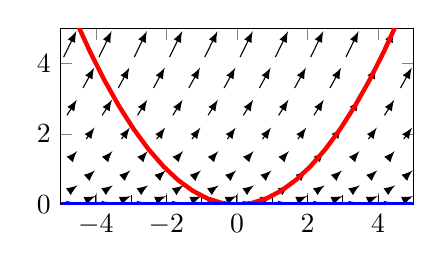
\begin{tikzpicture}[
	    			declare function={f(\x,\z) = (\x+\z)^2/4;}
			]
				\begin{axis}[
					width=0.5\textwidth, % Overall width of the plot
			        axis equal image, % Unit vectors for both axes have the same length
			        xmin=-5, xmax=5, % Axis limits
			        ymin=0, ymax=5,
			        domain=-5:5,
			        xtick={-4,-2,0,2,4}, ytick={0,2,4},
				]
					\foreach \z in {-5,...,9}
						\addplot[
							domain=-\z:-\z+5,
							samples=12,
							quiver={
			                    u={abs(x+\z)/2}, v={f(x,\z)*sign(x+\z)}, % End points of the arrows,
			                    scale arrows=0.175,
			                    every arrow/.append style={
			                        -latex % Arrow tip
			                    },
			                }]{f(\x,\z)};
			        \addplot[ultra thick, red]{f(x,0)};
			        \addplot[ultra thick, blue]{f(0,0)};
-				\end{axis}
			\end{tikzpicture}
			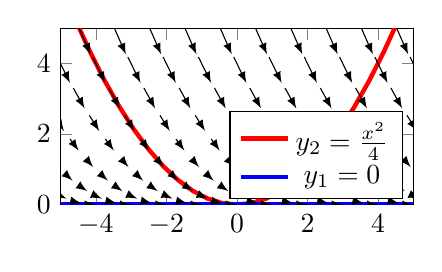
\begin{tikzpicture}[
	    			declare function={f(\x,\z) = (\x+\z)^2/4;}
			]
				\begin{axis}[
					width=0.5\textwidth, % Overall width of the plot
			        axis equal image, % Unit vectors for both axes have the same length
			        xmin=-5, xmax=5, % Axis limits
			        ymin=0, ymax=5,
			        domain=-5:5,
			        xtick={-4,-2,0,2,4}, ytick={0,2,4},
			        legend pos=south east
				]
					\addplot[ultra thick, red]{f(x,0)};
		            \addplot[ultra thick, blue]{f(0,0)};
					\foreach \z in {-9,...,5}
						\addplot[
							domain=-5-\z:-\z,
							samples=12,
							quiver={
			                    u={abs(x+\z)/2}, v={f(x,\z)*sign(x+\z)}, % End points of the arrows
			                    scale arrows=0.175,
			                    every arrow/.append style={
			                        -latex % Arrow tip
			                    },
			                }]{f(\x,\z)};
		                
		             \addlegendentry{$y_2=\frac{x^2}{4}$}
		             \addlegendentry{$y_1=0$}
				\end{axis}
			\end{tikzpicture}
			
			\item Erfüllt die rechte Seite von (*) eine Lipschitz-Bedingung?
			
			\begin{eqnn}
				\eqntext{$L\ge0$}
				\geqn[][]{f(y)-f(z)}{\le}{L|y-z|}
				\geqn[][]{\sqrt{y}-\sqrt{z}}{\le}{L|y-z|}
				\eqntext{ist immer Wahr für $y<z$, da linke Seite negativ wird}

				\geqn[][y>z:]{\sqrt{y}-\sqrt{z}}{\le}{L(\sqrt{y}-\sqrt{z})(\sqrt{y}+\sqrt{z})}
				\geqn[][y>z:]{1}{\le}{L(\sqrt{y}+\sqrt{z})}
				
			\end{eqnn}\\
		
		Da $\sqrt{y}+\sqrt{z}$ beliebig klein werden kann, gibt es $y,z$ Werte für die die Lipschitz-Bedingung nicht erfüllt wird.
		\end{enumerate}
		
		\item[8.5] Bestimme die allgemeine Lösung des Differentialgleichungssystems $y'=\begin{pmatrix}
			1&2\\
			3&2
		\end{pmatrix}y.$\\
		Berechne die Lösung zum Anfangswert $y(0)=\begin{pmatrix}
			1\\
			0
		\end{pmatrix}$
	
	\begin{eqnn}
		\eqntext{Eigenwerte bestimmen:}
		\eqn[][]{\begin{gmatrix}[v]
				1-\lambda&2\\
				3&2-\lambda
			\end{gmatrix}}{0}
		\eqn{(1-\lambda)(2-\lambda)-6}{0}
		\eqn{-4-3\lambda+\lambda^2}{0}
		\eqntext{$\Rightarrow$ $\lambda_1=4$, $\lambda_2=-1$}
		\eqntext{Eigenvektoren bestimmen:}
		\geqn[][]{v_1}{:}{\begin{gmatrix}[p]
				-3&2\\
				3&-2
		\end{gmatrix}}
		\eqn[][\Rightarrow]{v_1}{\begin{gmatrix}[p]
				2\\
				3
		\end{gmatrix}}
		\geqn[][]{v_2}{:}{\begin{gmatrix}[p]
			2&2\\
			3&3
		\end{gmatrix}}
		\eqn[][\Rightarrow]{v_2}{\begin{gmatrix}[p]
				1\\
				-1
		\end{gmatrix}}
		
		\eqntext{Lösungsansatz $y=e^{t\lambda}v$:}
		\eqn[][\Rightarrow]{y}{c_1e^{4t}\begin{gmatrix}[p]2\\3\end{gmatrix}+c_2e^{-t}\begin{gmatrix}[p]1\\-1\end{gmatrix}}
		\eqntext{Bedingung $y(0)=\begin{gmatrix}[p]1\\0\end{gmatrix}$ einsetzen:}
		\eqn[][]{\begin{gmatrix}[p]1\\0\end{gmatrix}}{\begin{gmatrix}[p]2&1\\3&-1\end{gmatrix}\begin{gmatrix}[p]c_1\\c_2\end{gmatrix}}
		\eqn{\frac{1}{5}\begin{gmatrix}[p]1\\3\end{gmatrix}}{\begin{gmatrix}[p]0&1\\1&0\end{gmatrix}\begin{gmatrix}[p]c_1\\c_2\end{gmatrix}}
		\eqntext{$\Rightarrow$ $c_1=\frac{1}{5}$ $c_2=\frac{3}{5}$}
		\eqn[][\Rightarrow]{y}{\frac{1}{5}\begin{gmatrix}[p]2&3\\3&-3\end{gmatrix}\begin{gmatrix}[p]e^{4t}\\e^{-t}\end{gmatrix}}
	\end{eqnn}
	\end{enumerate}
\end{document}
